% Template for Cogsci submission with R Markdown

% Stuff changed from original Markdown PLOS Template
\documentclass[10pt, letterpaper]{article}

\usepackage{cogsci}
\usepackage{pslatex}
\usepackage{float}
\usepackage{caption}

% amsmath package, useful for mathematical formulas
\usepackage{amsmath}

% amssymb package, useful for mathematical symbols
\usepackage{amssymb}

% hyperref package, useful for hyperlinks
\usepackage{hyperref}

% graphicx package, useful for including eps and pdf graphics
% include graphics with the command \includegraphics
\usepackage{graphicx}

% Sweave(-like)
\usepackage{fancyvrb}
\DefineVerbatimEnvironment{Sinput}{Verbatim}{fontshape=sl}
\DefineVerbatimEnvironment{Soutput}{Verbatim}{}
\DefineVerbatimEnvironment{Scode}{Verbatim}{fontshape=sl}
\newenvironment{Schunk}{}{}
\DefineVerbatimEnvironment{Code}{Verbatim}{}
\DefineVerbatimEnvironment{CodeInput}{Verbatim}{fontshape=sl}
\DefineVerbatimEnvironment{CodeOutput}{Verbatim}{}
\newenvironment{CodeChunk}{}{}

% cite package, to clean up citations in the main text. Do not remove.
\usepackage{cite}

\usepackage{color}

% Use doublespacing - comment out for single spacing
%\usepackage{setspace}
%\doublespacing


% % Text layout
% \topmargin 0.0cm
% \oddsidemargin 0.5cm
% \evensidemargin 0.5cm
% \textwidth 16cm
% \textheight 21cm

\title{When does passive learning improve the effectiveness of active learning?}


\author{{\large \bf Kyle MacDonald} \\ \texttt{kyle.macdonald@stanford.edu} \\ Department of   Psychology \\ Stanford University
    \And {\large \bf Michael C. Frank} \\ \texttt{mcfrank@stanford.edu} \\ Department of Psychology \\ Stanford University}

\begin{document}

\maketitle

\begin{abstract}
Much of what we learn comes from a mix of information that we select
(active) and information that we receive (passive). But which type of
training is better for different kinds of learning problems? Here, we
explore this question by comparing different sequences of active/passive
training in an abstract concept learning task. First, we replicate the
active learning advantage from Markant \& Gureckis (2014) (Experiments
1a and 1b). Then, we provide a test of whether experiencing active
learning first or passive learning first improves the effectiveness of
concept learning (Experiment 2). Across both experiments, active
training led to better learning of the target concept, but
``passive-first'' learners were more accurate than ``active-first''
learners and more efficient than ``active-only'' learners. These
findings broaden our understanding of when different sequences of
active/passive learning are more effective, suggesting that for certain
problems active exploration can be enhanced with prior passive
experience.

\textbf{Keywords:}
active learning, concept learning, replication
\end{abstract}

\section{Introduction}\label{introduction}

Much of real-world learning occurs in contexts that contain \emph{both}
active and passive input. People rarely learn a new concept entirely
from information generated by themselves (active learning\footnote{Here
  we focus on deliberate decisions about what to learn, as opposed to
  other uses of the term ``active'' learning (e.g., being engaged with
  learning materials).}) or entirely from information received from the
world (passive learning). And yet we do not have a theory about whether
different sequences of active/passive input are better for different
kinds of learning problems. Consider a teacher introducing a challenging
math concept: should she allow students to explore first and then
provide instruction, or should she teach first and then let students
actively explore?

The potential benefits of active learning have been the focus of much
research in education (Grabinger \& Dunlap, 1995), machine learning
(Settles, 2012), and cognitive science (Castro et al., 2009). In a
review of this diverse literature, Gureckis \& Markant (2012) suggest
that active learning can be superior to passive learning because it
allows people to use their prior experience and current hypotheses to
select the most helpful examples (e.g., asking a question about
something that is particularly confusing). But is active learning always
better than passive learning?

Gureckis \& Markant (2012) emphasize that the quality of active
exploration is fundamentally linked to the the learner's understanding
of the task: if the representation is poor, then self-directed learning
will be biased and ineffective. The potential for bias in active
learning suggests that receiving passive training first might be
especially important for less constrained learning tasks where people
are unlikely to generate examples that help them learn the target
concept. For example, work by Klahr \& Nigam (2004) shows that
elementary school-aged children are less effective at discovering the
principles of well-controlled experiments from their own self-directed
learning. Moreover, Markant \& Gureckis (2014) showed that active
exploration provided no benefit over passive input when there was a
mismatch between the target concept and learners' prior hypotheses. In
both of these cases, receiving passive training first might have
provided learners with a stronger task understanding that enhanced their
active exploration. In fact, recent work by Thai (2015) has shown that
receiving passive examples prior to performing active classifications
can enhance perceptual classification learning.

In contrast, experiencing active learning first might be better for
tasks with smaller problem spaces where helpful strategies can be
extracted via active exploration and generalized to the passive learning
context. Education research on the concept of \emph{productive failure}
shows that allowing students to struggle with a task (e.g.,
self-directed problem solving) can lead to better uptake of subsequent
instruction (Westermann \& Rummel, 2012). And work from cognitive
science shows that completing a block of active learning prior to
passive learning led to better word learning performance (Kachergis, Yu,
\& Shiffrin, 2013). Kachergis et al. (2013) suggest that active-first
learners were able to develop attention and memory strategies during
active training that generalized to the their passive learning
experience.

In the current work, we aim to provide a direct test of how different
sequences of active/passive training affect abstract category learning.
We use a well-understood perceptual category learning paradigm from
Markant \& Gureckis (2014) since this task produces a reliable active
learning advantage. We predicted that passive-first training would be
better than active-first training for two reasons. First, we thought
that people would generate hypotheses during passive learning, which
they could then refine with highly informative examples during active
exploration. Second, Markant \& Gureckis (2014) reported that the
quality of active learning was suboptimal early in their experiment,
presumably because people were building a better understanding of the
learning task. Thus, we predicted that providing passive learning first
would allow people to maximize the selection of high quality evidence
during active learning and improve their performance.

\begin{CodeChunk}
\begin{figure}[t]

{\centering 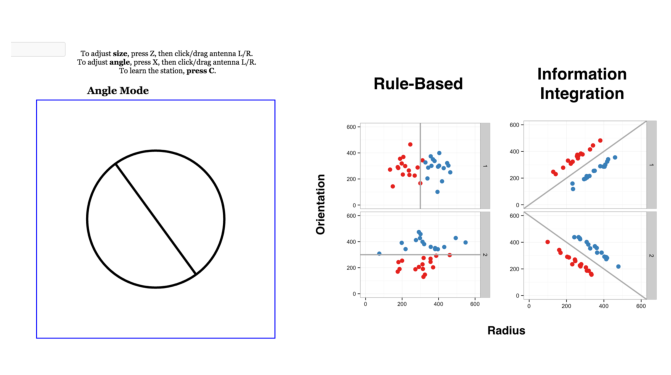
\includegraphics{figs/stimuli_exp1-1} 

}

\caption[An example of a training trial from the active learning condition in Experiments 1 and 2]{An example of a training trial from the active learning condition in Experiments 1 and 2. Participants could rotate the antenna or change the antenna's size before seeing which channel the antenna received.}\label{fig:stimuli_exp1}
\end{figure}
\end{CodeChunk}

\section{Experiment 1a}\label{experiment-1a}

Experiment 1a is a direct replication of the active learning advantage
for the Rule-Based (RB) category structure found in Markant \& Gureckis
(2014). In this task, people are asked to learn acategory boundary that
is defined by a point on a single continuous dimension (e.g., size).
Active learners generate their own examples, whereas passive learners
see data generated randomly from the category distributions. We used the
same stimuli and followed the exact procedures as the original study
with only minor differences, which we describe below. All of the
stimuli, the experiments, and analysis code can be viewed and downloaded
at the project page for this paper:
\url{https://kemacdonald.github.io/Act-Learn/}.

\subsection{Methods}\label{methods}

\subsubsection{Participants}\label{participants}

We planned a sample of 48 participants, 24 in each condition and posted
a set of Human Intelligence Tasks (HITs) to Amazon Mechanical Turk. Only
participants with US IP addresses and a task approval rate above 85\%
were allowed to participate, and each HIT paid one dollar. Data were
excluded if participants completed the task more than once or if they
reported to not understand the task at the end of the experiment (1
HITs). The final sample consisted of 52 participants (Passive: 27;
Active: 25).

\begin{CodeChunk}
\begin{figure}[t]

{\centering 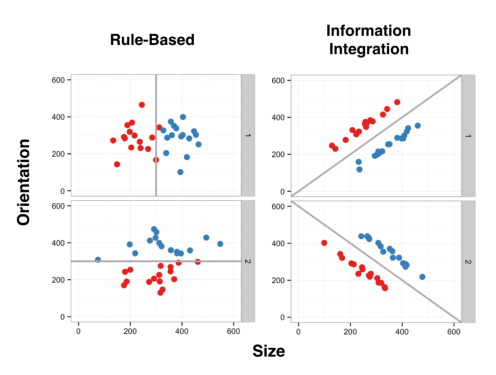
\includegraphics{figs/category_exp1-1} 

}

\caption[Example distributions of training stimuli shown to participants in the passive learning condition]{Example distributions of training stimuli shown to participants in the passive learning condition. Each point represents a different antenna constructed with an orientation value (vertical axis) and radius value (horizontal axis). The color of the points show the category membership of each antenna (red: channel 1; blue: channel 2). The solid line in each facet represents the optimal category boundary for both the Rule-Based category and the Information-Integration category structures.}\label{fig:category_exp1}
\end{figure}
\end{CodeChunk}

\begin{CodeChunk}
\begin{figure*}[t]

{\centering 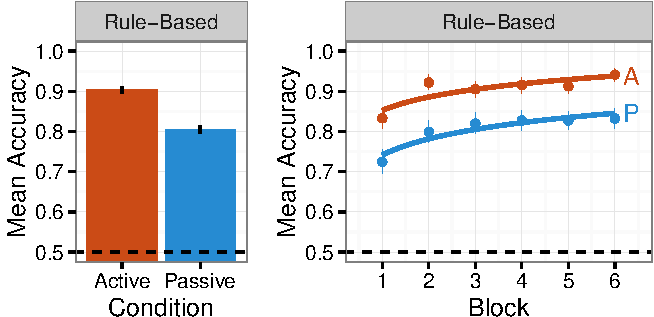
\includegraphics{figs/exp1a_acc_plot-1} 

}

\caption[The left panel shows overall accuracy performance on the classification task for the Active and Passive training conditions from Experiment 1a]{The left panel shows overall accuracy performance on the classification task for the Active and Passive training conditions from Experiment 1a. The right panel shows accuracy across each of the six blocks in the experiment. The grey curves are generated by a logarithmic smoother and the error bars indicate 95\% confidence intervals computed by non-parametric bootstrap.}\label{fig:exp1a_acc_plot}
\end{figure*}
\end{CodeChunk}

\subsubsection{Stimuli}\label{stimuli}

Visual stimuli were black ``antennas'' on a white background (Fig 1).
Each antenna could vary along two continuous dimensions -- radius size
or central angle -- and was assigned a value between 1-600. To make sure
that participants could not completely rotate the antenna, we limited
the rotation to 150 degrees. The smallest radius and angle parameter
values were randomized for each participant, so each participant had a
unique category boundary. Finally, we used the Rule-Based category
structure where the category boundary is defined by a point on a single
dimension: either size or central angle.

Radius and angle values for the 96 passive training trials were
generated from two Gaussian distributions with identical mean and
covariance parameters as Markant \& Gureckis (2014) (Fig 2). For test
trials, we created a uniform grid of 192 unique test items that covered
the entire parameter space. We randomly sampled 8 items from each
quadrant to get 32 test trials for each block and randomized the order
of training and test trials within each block and for each participant.

\subsubsection{Design and procedure}\label{design-and-procedure}

Participants saw a total of 288 trials (96 training and 192 test trials)
across 6
blocks\footnote{Six blocks is two blocks shorter than the original experiment. We reduced the length to increase our sample size.}.
Each block consisted of 16 training and 32 test trials. Before the task,
participants were told that they would see ``loop antennas'' for
televisions and each antenna received one of two channels, and their
goal was to learn the difference between the two types of antennas. We
told participants that the antennas could sometimes pick up the wrong
channel, and that they should learn what channel is most often received
by a particular type of antenna.

After the instructions, participants were randomly assigned to one of
the two between-subjects conditions (Active vs.~Passive). In the Active
condition, participants could design their own antennas. They modified
the antenna by clicking and dragging the mouse from left to right. To
change the size of the antenna, they first pressed the ``Z'' key. To
change the angle, they first pressed the ``X'' key. When participants
were finished with their design, they pressed the space bar to see which
channel the antenna received. The channel label appeared in a text box
with a green border located above the antenna.

In the Passive condition, participants saw antennas generated randomly
using the size and angle values taken from the category distributions.
After a two second delay they were told which channel the antenna
received. The channel labels were deterministic. To help ensure that
participants actually saw the channel, they had to click on the channel
label in order to advance the experiment. When they clicked, a green box
appeared around the text to indicate that their response was recorded.

After training, participants proceeded to test trials. On each test
trial participants saw one antenna and were asked, ``Which channel does
this antenna receive?'' To indicate their response, participants
selected one of two buttons (Ch1 or Ch2) located above the antenna. At
the end of each block of test trials, participants saw a summary of
their accuracy on the preceding block.

\subsection{Results and Discussion}\label{results-and-discussion}

\subsubsection{Classification accuracy}\label{classification-accuracy}

First we report the planned replication analysis: a t-test to compare
overall classification performance between the active and passive
conditions. Active learners were more accurate, \(t\)(49) = 2.98, \(p\)
= 0.004. Moreover, the effect size of the active learning advantage was
large and greater than that of the original study (Original study: \(d\)
= 0.47; Replication: \(d\) = 0.73).

\subsubsection{Classification accuracy over
time}\label{classification-accuracy-over-time}

To quantify performance over time, we used a mixed effect logistic
regression including a random effect for participants. We predicted test
performance at the trial-level as a function of condition
(Active/Passive) and block (1-6) and found a main effect of condition
(\(\beta\) = -0.68, \(p\) = 0.041) with better performance for active
learners overall, and a main effect of block (\(\beta\) = 0.25, \(p\)
\textless{} .001) such that responses were more accurate later in the
experiment. There was also an interaction between block and condition
(\(\beta\) = -0.1, \(p\) = 0.01) with passive learners showing less of
an increase in accuracy across the six test blocks.

\subsubsection{Relations between quality of active learning and
accuracy}\label{relations-between-quality-of-active-learning-and-accuracy}

Another important result from Markant \& Gureckis (2014) was the link
between the quality of active learning and classification accuracy.
Thus, we performed the same analysis on our replication data,
quantifying the quality of evidence selection by computing the
orthogonal distance between each sample and the true category boundary.
Samples closer to the boundary are higher quality. We computed a mean
accuracy score and a mean sample distance score for each participant,
and fit a linear model using the mean sample distance score to predict
accuracy. We found an effect of sample distance (\(\beta\) = -.0004, p
\textless{} .001) with accuracy increasing as the sample distance
decreased.

Experiment 1a provides strong evidence for a successful replication of
the original results reported in Markant \& Gureckis (2014). We found a
comparable advantage in accuracy for active learners and we found the
same relationship between quality of evidence selection and learning
outcomes. Our results differ slightly from the original study in that we
found an immediate advantage for active learners in the first block. We
next attempt to replicate Markant \& Gureckis (2014)'s findings for the
more complex Information-Integration category structure and for the
yoked passive learning condition.

\section{Experiment 1b}\label{experiment-1b}

The goals of Experiment 1b were: (a) to replicate the lack of an active
learning advantage for the more difficult Information-Integration (II)
category structure, where the category boundary was defined by a linear
combination of an antenna's size and central angle, and (b) to replicate
the finding that passive learners did not benefit from being ``yoked''
to active learners' data. We also performed an internal replication of
the active learning advantage for the RB category that we found in
Experiment 1a. We used the same stimuli and followed the exact
procedures as the original study. However, we reduced the length of the
experiment to two blocks in order to increase our sample size.

\begin{CodeChunk}
\begin{figure}[t]

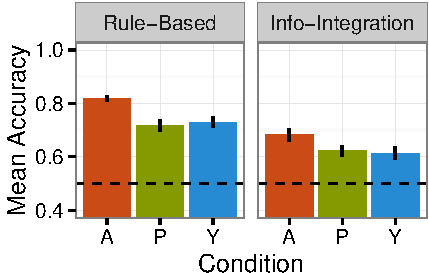
\includegraphics{figs/rep1b-acc-plot-1} \hfill{}

\caption[Accuracy across each of the two blocks in Experiment 1b for the Active, Passive, and Yoked training conditions for the Rule-Based (one dimension) and Information-Integration (two dimensions) category structures]{Accuracy across each of the two blocks in Experiment 1b for the Active, Passive, and Yoked training conditions for the Rule-Based (one dimension) and Information-Integration (two dimensions) category structures. Error bars indicate 95\% confidence intervals computed by non-parametric bootstrap.}\label{fig:rep1b-acc-plot}
\end{figure}
\end{CodeChunk}

\subsection{Methods}\label{methods-1}

\subsubsection{Stimuli}\label{stimuli-1}

Visual stimuli were identical to Experiment 1a.

\subsubsection{Participants}\label{participants-1}

Participant recruitment and inclusionary/exclusionary criteria were
identical to those of Experiment 1a (excluded 3 HITs). 196 HITs were
posted across each of the between-subjects conditions: two category
structures and three training conditions (A-RB: 66, A-II: 26, P-RB: 25,
P-II: 28, Y-RB: 27, and Y-II: 24).

\subsubsection{Design and procedure}\label{design-and-procedure-1}

Procedures were identical to those of Experiment 1a except that we
included a ``yoked'' learning condition where we matched each passive
learning participant with training data generated by an active learner.
Thus, the active and yoked participants saw the exact same data, but
active learners were in control of the information flow. We also reduced
the length of the experiment to two blocks.

\begin{CodeChunk}
\begin{figure}[t]

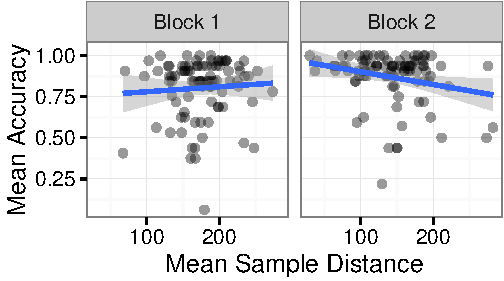
\includegraphics{figs/samp_acc_scatter_plot-1} \hfill{}

\caption[The relations between quality of evidence selection and accuracy on test trials across blocks for participants in Experiments 1a and 1b]{The relations between quality of evidence selection and accuracy on test trials across blocks for participants in Experiments 1a and 1b. Each point is an individual participant. Note that higher mean sample distance means worse evidence selection. The blue lines are linear model fits.}\label{fig:samp_acc_scatter_plot}
\end{figure}
\end{CodeChunk}

\begin{CodeChunk}
\begin{figure}[h]

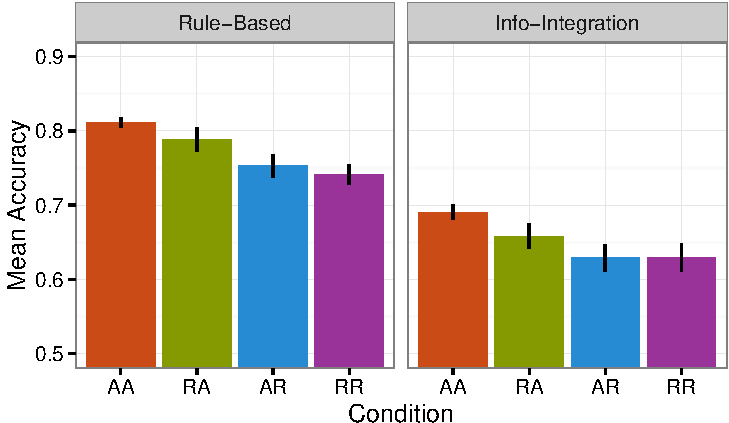
\includegraphics{figs/exp2_acc_plot-1} \hfill{}

\caption[Accuracy across each of the two blocks in Experiment 2 for the Passive-Active (PA) and Active-Passive (AP) conditions for the Rule-Based (one dimension) and Information-Integration (two dimensions) category structures]{Accuracy across each of the two blocks in Experiment 2 for the Passive-Active (PA) and Active-Passive (AP) conditions for the Rule-Based (one dimension) and Information-Integration (two dimensions) category structures. Error bars indicate 95\% confidence intervals computed by non-parametric bootstrap.}\label{fig:exp2_acc_plot}
\end{figure}
\end{CodeChunk}

\subsection{Results and Discussion}\label{results-and-discussion-1}

\subsubsection{Classification accuracy}\label{classification-accuracy-1}

We fit the same logistic regression as specified in Experiment 1a and
found a main effect of category (\(\beta\) = -0.82, p \textless{} .001)
with better performance in the RB category. We also found a main effect
of condition (\(\beta\) = -0.76, p \textless{} .001) such that
participants in the passive and yoked conditions performed worse than
participants in the active condition. We also found an interaction
between block and the passive learning condition (\(\beta\) = 0.33,
\(p\) = 0.03) with passive learners showing more learning over time, and
an interaction between category type and block (\(\beta\) = -0.29, \(p\)
= 0.04) with less learning in the II category.

\subsubsection{Relations between evidence selections and accuracy over
time}\label{relations-between-evidence-selections-and-accuracy-over-time}

Since the main goal of the current work was to test the effectiveness of
different sequences of active/passive learning, we performed an
exploratory analysis of the relations between sampling behavior and test
accuracy over time for all active learners in Experiments 1a and 1b. We
fit a linear model predicting each participant's mean accuracy based on
the quality of their sampling behavior and experiment block. As
expected, participants' accuracy improved in the second block (\(\beta\)
= 0.21, \(p\) = 0.01). Interestingly, there was a reliable two-way
interaction between sample distance and block (\(\beta\) = -0.0013,
\(p\) = 0.005) such that the relationship between the quality of
evidence selection and accuracy did not emerge until the second block
(see Fig 5).

Experiment 1b provides additional evidence for a successful replication
of the original results reported in Markant \& Gureckis (2014).
Importantly, yoked learners performed worse than active learners even
though they had seen the same training data, suggesting that the link
between people's hypotheses and the input is an important contributor to
the active learning advantage. We did find that active learners
performed better than both passive and yoked learners in the more
complex II category structure. This advantage was not found in the
original study, but this finding fits with recent work by Edmunds,
Milton, \& Wills (2015) suggesting that RB and II categories are not
learned in qualitatively different ways. Finally, we found evidence that
the link between the quality of active learning and accuracy emerges as
people gain more experience with the task -- an effect that we set out
to explore in Experiment 2.

\section{Experiment 2}\label{experiment-2}

Direct comparisons of active and passive learning are important for
understanding when and why we might see advantages for one type of
learning over the other. But real-world contexts are not neatly divided
into active learning and passive learning. So when are different kinds
of learning better for different kinds of learning problems? Experiment
2 provides a direct test of different predictions about the effects of
different sequences of active/passive training in an abstract category
learning task. Is active-first learning better because it makes people
to engage more deeply with the task, enhancing their subsequent passive
learning? Or is passive-first training better because it enhances later
active learning?

\subsection{Methods}\label{methods-2}

\subsubsection{Stimuli}\label{stimuli-2}

Stimuli were identical to Experiment 1.

\subsubsection{Participants}\label{participants-2}

Participant recruitment and inclusionary/exclusionary criteria were
identical to those of Experiment 1 (3 HITs). Approximately 44 HITs were
posted for each training condition and category type for total of 176
paid HITs (AR-RB: 46, AR-II: 41, RA-RB: 38, RA-II: 51).

\subsubsection{Design and procedure}\label{design-and-procedure-2}

Procedures were identical to those of Experiment 1. Participants were
randomly assigned to one the two between-subjects conditions:
Active-Passive (AP) vs.~Passive-Active (PA). In the AP condition,
participants completed a block of active training and test trials before
proceeding to a block of passive learning and test trials. In the PA
condition, the order of the training/test blocks was reversed with
passive training coming first.

\subsection{Results and Discussion}\label{results-and-discussion-2}

First, we present analyses of classification accuracy and sampling
behavior, focusing on just the AP and PA conditions. The key test of our
hypothesis is the interaction between training condition and experiment
block, since this tests the effect of training condition on improvement
in classification accuracy. We then compare performance in the AP and PA
conditions to performance from the Active-Active (AA) and
Passive-Passive (PP) conditions from Experiments 1a and 1b, which allows
for comparisons to training regimes where learners did not have to
switch between types of learning.

\subsubsection{Classification accuracy}\label{classification-accuracy-2}

Which sequence of active and passive learning was better? We fit a
logistic regression predicting test performance based on condition (PA
vs.~AP), block (1 vs.~2), and category type (RB vs.~II). We found a main
effect of block (\(\beta\) = 0.63, p \textless{} .001), with better
performance in the second block across all conditions. For the key test
of our hypothesis, we found a reliable two-way interaction between
training condition and block (\(\beta\) = -0.39, p \textless{} .001),
such that participants in the PA condition showed more learning over
time compared to the AP condition. We also found a reliable two-way
interaction between category type and block (\(\beta\) = -0.44, p
\textless{} .001) and a marginally significant three-way interaction
between condition, category type, and block (\(\beta\) = 0.32, \(p\) =
0.08). Participants showed less of an increase in accuracy for the more
complex II category, and there was less of an advantage for the PA
training condition in the II category.

\subsubsection{Quality of evidence
selection}\label{quality-of-evidence-selection}

To test which condition produced higher quality sampling behavior, we
fit a linear mixed model predicting sample quality as a function of
condition and category type. We found that PA learners generated better
samples than AP learners (\(\beta\) = 22.4, \(t\) = 2.3), and we found
that sampling quality was lower in the II category (\(\beta\) = 61.08,
\(t\) = 6.46). We also we fit a linear model predicting mean
classification accuracy based on the mean distance of samples from the
target category boundary, and replicate the finding from Experiments 1a
and 1b: that higher quality sampling was related to higher accuracy
scores (\(\beta\) = .00006, \(p\) = 0.01).

\subsubsection{Classification accuracy for all
sequences}\label{classification-accuracy-for-all-sequences}

How does learning from different sequences of active/passive learning
compare to learning from only active or passive data? We fit a logistic
regression predicting test performance with the same specifications, but
we included data from the active and passive learning conditions in
Experiments 1a and 1b and coded user-defined contrasts to test
classification accuracy for specific comparisons of interest. We found
that receiving any active learning (AA, PA, AP) was better than
receiving only passive learning (PP) (\(\beta\) = 0.07, \(p\)
\textless{} .01), and that completing two blocks of active learning (AA)
was marginally better than completing one block of active learning (PA
or AP) (\(\beta\) = 0.06, \(p\) = 0.09).

\subsubsection{Time costs associated with different learning
sequences}\label{time-costs-associated-with-different-learning-sequences}

We were also interested in the time costs associated with different
sequences of active and passive learning. We fit a linear mixed effects
model with the same specifications but predicting the amount of time
spent on each training trial. We found that training took longer in any
active learning condition compared to passive learning (\(\beta\) =
2.59, \(t\) = 11.57). We also found that people who completed only
active training (AA) took longer than people who only completed one
block of active learning (PA, AP) (\(\beta\) = -0.71, \(t\) = -2.22).
Surprisingly, we found that people in the active-first condition (AP)
took longer than people in the passive-first condition (PA) (\(\beta\) =
2.67, \(t\) = 3.64). We did not find any reliable interactions.

The main findings from Experiment 2 are that despite experiencing the
exact same amount of active and passive data, passive-first learners
were more accurate overall, produced higher quality sampling behavior,
and spent less time on training. These results suggest that receiving
passive training first improved learners' active learning by helping
them to explore more efficiently.

\section{General Discussion}\label{general-discussion}

Mixtures of active and passive learning are a fundamental feature of
real-world learning contexts. But we do not know when different
sequences of active/passive input are better for different kinds of
learning problems. In the current work, we take a first step towards
answering this important question. We found that that receiving passive
learning first improved subsequent active exploration and led to better
overall performance in an abstract concept learning task. This finding
broadens our understanding of the types of learning problems where
passive learning might support effective active learning.

Why was passive-first learning better in this kind of abstract concept
learning problem? One possibility is passive training allowed people to
generate hypotheses about the correct category boundary, which they
could begin testing from the very first trial of active learning. We did
find that passive-first learners produced higher quality active
learning, suggesting that perhaps active-first learners used their
initial active learning less effectively. In contrast, we did not see
active learning strategies transfer to passive learning, as had been
found previously (Kachergis et al., 2013). Perhaps we did not see
transfer because this task involved incremental changes to hypotheses,
which depend on generating the right example to falsify the learner's
current hypothesis on a trial by trial basis. In contrast, if active
learning helps learners develop better attentional/memory strategies,
these strategies can often be transferred to passive contexts.

It is interesting that two blocks of active learning was slightly better
than the passive-first learning. But, passive-first learning provides an
additional benefit: it reduces learning costs (i.e., time and mental
effort). We found that active learners took longer to complete the task
and spent more time on the training blocks. Thus, even if passive-first
learning does not achieve the same level of performance as active
learning, it still might be preferable.

There are several limitations to our experiment. First, while the
learning task we used is well-understood, like other tasks of this type
it dramatically simplifies real-world concept learning. So we do not
know how our sequencing finding would scale to learning more complex,
higher dimensional concepts. It could be that passive learning becomes
even more important as the concept becomes more complex. Second, we used
a coarse sequence manipulation, at the level of training/test blocks.
And sequences of active/passive learning might have differential effects
on learning at finer levels of granularity (e.g., trial level).

We need a theory of what kinds of learning work best for the diverse set
of problems that learners must solve. Our work here provides an
important first step towards understanding when passive learning
experiences could be used to support better active exploration. Overall,
these results show that, for some tasks, passive learning can equip
people with a better task representation, making them more effective
active learners.

\section{Acknowledgements}\label{acknowledgements}

We are grateful to Doug Markant and Todd Gureckis for sharing the
details and code from the original experiment. We thank the members of
the Language and Cognition Lab for their helpful feedback on this
project. This work was supported by a National Science Foundation
Graduate Research Fellowship to KM.

\section{References}\label{references}

\setlength{\parindent}{-0.1in} \setlength{\leftskip}{0.125in} \noindent

Castro, R. M., Kalish, C., Nowak, R., Qian, R., Rogers, T., \& Zhu, X.
(2009). Human active learning. In \emph{Advances in neural information
processing systems} (pp. 241--248).

Edmunds, C., Milton, F., \& Wills, A. J. (2015). Feedback can be
superior to observational training for both rule-based and
information-integration category structures. \emph{The Quarterly Journal
of Experimental Psychology}, \emph{68}(6), 1203--1222.

Grabinger, R. S., \& Dunlap, J. C. (1995). Rich environments for active
learning: A definition. \emph{Research in Learning Technology},
\emph{3}(2).

Gureckis, T. M., \& Markant, D. B. (2012). Self-directed learning a
cognitive and computational perspective. \emph{Perspectives on
Psychological Science}, \emph{7}(5), 464--481.

Kachergis, G., Yu, C., \& Shiffrin, R. M. (2013). Actively learning
object names across ambiguous situations. \emph{Topics in Cognitive
Science}, \emph{5}(1), 200--213.

Klahr, D., \& Nigam, M. (2004). The equivalence of learning paths in
early science instruction effects of direct instruction and discovery
learning. \emph{Psychological Science}, \emph{15}(10), 661--667.

Markant, D. B., \& Gureckis, T. M. (2014). Is it better to select or to
receive? Learning via active and passive hypothesis testing.
\emph{Journal of Experimental Psychology: General}, \emph{143}(1), 94.

Settles, B. (2012). Active learning. \emph{Synthesis Lectures on
Artificial Intelligence and Machine Learning}, \emph{6}(1), 1--114.

Thai, K.-P. (2015). Making experts: Optimizing perceptual learning in
complex, real-world learning domains.

Westermann, K., \& Rummel, N. (2012). Delaying instruction: Evidence
from a study in a university relearning setting. \emph{Instructional
Science}, \emph{40}(4), 673--689.

\end{document}
